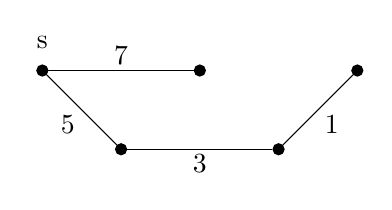
\begin{tikzpicture}[black/.style={circle,draw,fill=black,inner sep=0pt, minimum width=4pt}]
\foreach \x/\y in {1,3,5}
	\node[black] at (\x,1) (\x) {};
\foreach \x in {2,4}
	\node[black] at (\x,0) (\x) {};


\node[yshift=10] at (1,1) () {s};

\draw (1) -- (3) node [midway, label={7},yshift=-5] {};;
% \draw (3) -- (5) node [midway, label={3},yshift=-5] {};);
\draw (2) -- (4) node [midway, label=below:{3},yshift=5] {};);

\draw (1) -- (2) node [midway, label=below:{5},xshift=-5,yshift=5] {};);
% \draw (2) -- (3) node [midway, label={8},xshift=-5,yshift=-5] {};);
% \draw (3) -- (4) node [midway, label={2},xshift=5,yshift=-5] {};);
\draw (4) -- (5) node [midway, label=below:{1},xshift=5,yshift=5] {};);
\end{tikzpicture}
